\documentclass[11pt]{article}
\usepackage[margin=1in]{geometry}
\usepackage{clrscode3e}
\usepackage{amsmath,amsthm,amssymb}
\usepackage{mathtools}
\usepackage{tikz}
\usepackage{float}
\usetikzlibrary{positioning,arrows}
\usepackage{setspace}
\usepackage{mathpazo}
\doublespacing
%\usepackage{tikz-berge}
%\usepackage{algorithm}
%\usepackage[noend]{algpseudocode}

 
\newcommand{\N}{\mathbb{N}}
\newcommand{\Z}{\mathbb{Z}}
\newcommand{\R}{\mathbb{R}}
\renewcommand{\'}{^{'}}
\renewcommand{\gets}{:=}
 
\newenvironment{theorem}[2][Theorem]{\begin{trivlist}
\item[\hskip \labelsep {\bfseries #1}\hskip \labelsep {\bfseries #2.}]}{\end{trivlist}}
\newenvironment{lemma}[2][Lemma]{\begin{trivlist}
\item[\hskip \labelsep {\bfseries #1}\hskip \labelsep {\bfseries #2.}]}{\end{trivlist}}
\newenvironment{definition}[2][Definition]{\begin{trivlist}
\item[\hskip \labelsep {\bfseries #1}\hskip \labelsep {\bfseries #2.}]}{\end{trivlist}}
\newenvironment{problem}[2][Problem]{\begin{trivlist}
\item[\hskip \labelsep {\bfseries #1}\hskip \labelsep {\bfseries #2.}]}{\end{trivlist}}
\newenvironment{question}[2][Question]{\begin{trivlist}
\item[\hskip \labelsep {\bfseries #1}\hskip \labelsep {\bfseries #2.}]}{\end{trivlist}}

\begin{document}
\title{Chapter 2}
\author{Zachary Campbell}

\maketitle

\begin{section}{The Hungarian algorithm}
	In this section we use the motivation of the linear programs to develop an algorithm for 
	simultaneously solving the maximum weight matching and minimum weight vertex cover problems.
	Our algorithm works by taking every exposed node on the left, and from each such  node building 
	a collection of alternating paths. We define this collection formally.
	\begin{definition}{(Alternating tree)}
		Let $G = (U,V,E)$ be a bipartite graph, and $M$ a matching on $G$. An 
		\emph{alternating tree} with respect to $M$ is a tree which satisfies two 
		conditions:
		\begin{itemize}
			\item the tree contains exactly one node $u\in U$. We call $u$ the 
				\emph{root} of the tree.
			\item all paths between the root and any other node in the tree are 
				alternating paths.
		\end{itemize}
	\end{definition}
	\begin{figure}[h]
		\centering
		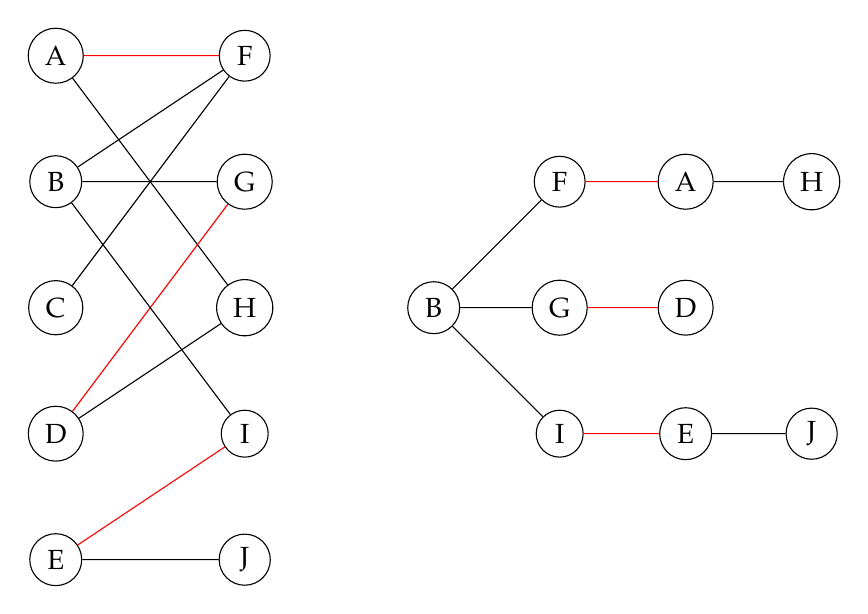
\begin{tikzpicture}[scale=.8,auto=left,every node/.style={circle,draw=black}]
		
		%left nodes
		\node (n1) at (1,10) {A};
		\node (n2) at (1,8) {B};
		\node (n3) at (1,6) {C};
		\node (n4) at (1,4) {D};
		\node (n5) at (1,2) {E};

		%right nodes
		\node (n6) at (4,10) {F};
		\node (n7) at (4,8) {G};
		\node (n8) at (4,6) {H};
		\node (n9) at (4,4) {I};
		\node (n10) at (4,2) {J};
		
		%edges
		\draw[red] (n1) -- (n6);
		\draw (n1) -- (n8);
		\draw (n2) -- (n6);
		\draw (n2) -- (n7);
		\draw (n3) -- (n6);
		\draw[red] (n4) -- (n7);
		\draw (n4) -- (n8);
		\draw (n2) -- (n9);
		\draw[red] (n5) -- (n9);
		\draw (n5) -- (n10);

		%alternating tree
		\node (n11) at (7,6) {B};
		\node (n12) at (9,8) {F};
		\node (n13) at (9,6) {G};
		\node (n14) at (9,4) {I};
		\node (n15) at (11,8) {A};
		\node (n16) at (11,6) {D};
		\node (n17) at (11,4) {E};
		\node (n18) at (13,8) {H};
		\node (n20) at (13,4) {J};

		%tree edges
		\draw (n11) -- (n12);
		\draw (n11) -- (n13);
		\draw (n11) -- (n14);
		\draw[red] (n12) -- (n15);
		\draw[red] (n13) -- (n16);
		\draw[red] (n14) -- (n17);
		\draw (n15) -- (n18);
		\draw (n17) -- (n20);
		\end{tikzpicture}
		\caption{Bipartite graph with matching, corresponding alternating tree rooted at 
		vertex $B$.}
	\end{figure}
	Let's remind ourselves what the primal-dual linear programs
	motivate. We want to minimize $\sum w_{uv}$, and maximize $\sum (y_u + y_v)$. Moreover, 
	we want optimal solutions such that $\sum w_{uv} = \sum (y_u + y_v)$. For our primal, we are 
	keeping track of edge weights. For the dual, we will be keeping track of a ``labeling'' on 
	vertices, given by the $y_u$ and $y_v$ values. We define what a labeling is now.

	\begin{definition}{(Labeling)}
		A \emph{vertex labeling} on a weighted bipartite graph $G = (U,V,E)$ is a function 
		$l: U\cup V \to \N$. We call the labeling \emph{feasible} if for all $u\in U$ and 
		$v\in V$, $l(u) + l(v) \geq w_{uv}$.
	\end{definition}
	This labeling corresponds to our dual variables; i.e. a feasible labeling is a feasible dual 
	solution. It will be helpful us to look at a certain subset of our graph where the labeling 
	is exact ($l(u) + l(v) - w_{uv} = 0$).
	\begin{definition}{(Equality subgraph)}
		The \emph{equality subgraph} of $G = (U,V,E)$ is the graph $G_l = (U,V,E_l)$, 
		where 
		\[
			E_l = \{(u,v)\ :\ l(u) + l(v) = w_{uv}\}.
		\]
	\end{definition}
	In Figure 5 we show a bipartite graph along with its corresponding equality graph.
	\begin{figure}[h]
		\centering
		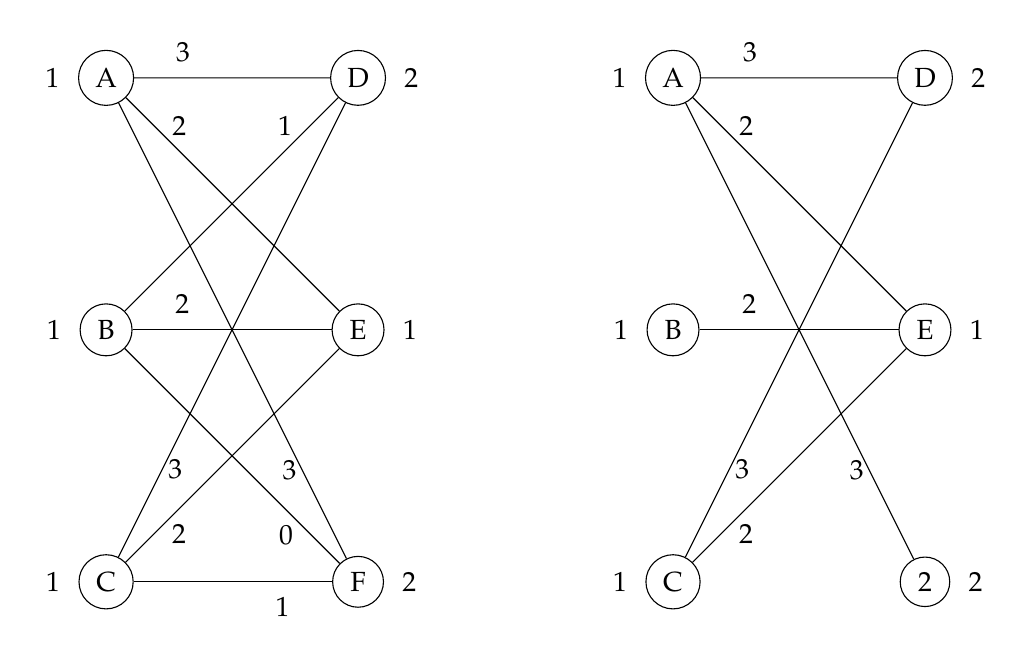
\begin{tikzpicture}[scale=.8,auto=left,every node/.style={circle,draw=black}]
			%left nodes
			\node [label=left:{1}] (n1) at (1,10) {A};
			\node [label=left:{1}] (n2) at (1,6) {B};
			\node [label=left:{1}] (n3) at (1,2) {C};

			%right nodes
			\node [label=right:{2}] (n4) at (5,10) {D};
			\node [label=right:{1}] (n5) at (5,6) {E};
			\node [label=right:{2}] (n6) at (5,2) {F};

			%edges
			\draw (n1) -- node[near start,draw=none,above] {3} ++(n4);
			\draw (n1) -- node[near start,draw=none,above] {2} ++(n5);
			\draw (n1) -- node[near end,draw=none,below] {3} ++(n6);

			\draw (n2) -- node[near end,draw=none,above] {1} ++(n4);
			\draw (n2) -- node[near start,draw=none,above] {2} ++(n5);
			\draw (n2) -- node[near end,draw=none,below] {0} ++(n6);

			\draw (n3) -- node[near start,draw=none,below] {3} ++(n4);
			\draw (n3) -- node[near start,draw=none,below] {2} ++(n5);
			\draw (n3) -- node[near end,draw=none,below] {1} ++(n6);


			%left nodes
			\node [label=left:{1}] (n7) at (10,10) {A};
			\node [label=left:{1}] (n8) at (10,6) {B};
			\node [label=left:{1}] (n9) at (10,2) {C};

			%right nodes
			\node [label=right:{2}] (n10) at (14,10) {D};
			\node [label=right:{1}] (n11) at (14,6) {E};
			\node [label=right:{2}] (n12) at (14,2) {2};

			%edges
			\draw (n7) -- node[near start,draw=none,above] {3} ++(n10);
			\draw (n7) -- node[near start,draw=none,above] {2} ++(n11);
			\draw (n7) -- node[near end,draw=none,below] {3} ++(n12);

			\draw (n8) -- node[near start,draw=none,above] {2} ++(n11);

			\draw (n9) -- node[near start,draw=none,below] {3} ++(n10);
			\draw (n9) -- node[near start,draw=none,below] {2} ++(n11);
		\end{tikzpicture}
		\caption{A weighted bipartite graph and its corresponding equality subgraph.}
	\end{figure}
	\begin{theorem}{(Kuhn-Munkres)}
		If $l$ is a feasible labeling and $M$ is a perfect matching in $G_l$ then $M$ is a 
		max-weight matching.
	\end{theorem}

	\begin{proof}
		Let $M\'$ be a perfect matching in $G$. Since every $u\in U\cup V$ is matched 
		by exactly one edge in $M\'$, then 
		\[
			\sum_{(u,v)\in M\'} w_{uv} \leq \sum_{(u,v)\in M\'} (l(u)+l(v)) = 
			\sum_{w\in U\cup V} l(w).
		\]
		This says that the sum of our label values is an upper bound on the weight of any 
		perfect matching.
		Now suppose that $M$ is a perfect matching in $G_l$. Then 
		\[
			\sum_{(u,v)\in M} w_{uv} = \sum_{w\in U\cup V} l(w).
		\]
		So $\sum_{(u,v)\in M\'} w_{uv} \leq \sum_{(u,v)\in M}$, meaning $M$ must be maximum 
		weight.
	\end{proof}

	\begin{lemma}{2}
		Let $S\subseteq U$ and $T = N_l(S) \neq V$. Set 
		\[
			\alpha_l = \min _{u\in S,\ v\notin T} \{l(u) + l(v) - w_{uv}\}
		\]
		and 
		\[
			l\' (w) = 
			\begin{cases}
				l(w) - \alpha_l &\text{ if } w\in S \\
				l(w) + \alpha_l &\text{ if } w\in T \\
				l(w) &\text{ otherwise.}
			\end{cases}
		\]
		Then $l\'$ is a feasible labeling, and 
		\begin{enumerate}
			\item If $(u,v)\in E_l$ for $u\in S$ and $v\in T$ then $(u,v)\in E_{l\'}$.
			\item If $(u,v)\in E_l$ for $u\notin S$, and $v\notin T$, then $(u,v)\in 
				E_{l\'}$.
			\item There is some edge $(u,v)\in E_{l\'}$ for $u\in S$, $v\notin T$.
		\end{enumerate}
	\end{lemma}

	\begin{proof}
		First, we show that $l\'$ is feasible. For $u\in U$, $v\in V$, there are four 
		possibilities:
		\begin{itemize}
			\item if $u\in S$ and $v\in T$ then $l\' (u) + l\' (v) = l(u) + l(v)$.
			\item if $u\notin S$ and $v\notin T$, $l\' (u) = l(u)$ and $l\' (v) = l(v)$, 
				so $l\' (u) + l\' (v) = l(u) + l(v)$.
			\item if $u\in S$ and $v\notin T$, $l\' (u) - \alpha$ and $l\' (v) = l(v)$. 
				We know $\alpha = \min_{u\in S,v\notin T} \{l(u) + l(v) - w_{uv}\}$, 
				which means $\alpha \leq l(u) + l(v) - w_{uv}$, and thus 
				$l\' (u) + l\' (v) \geq w_{uv}$.
			\item if $u\notin S$ and $v\in T$, $l\' (u) = l(u)$ and $l\' (v) = l(v) + 
				\alpha$, which is clearly feasible.
		\end{itemize}
		(1) and (2) follow from above. To see (3), note that there is some $(u,v)$ with 
		$u\in S$, $v\in T$ such that $\alpha = l(u) + l(v) - w_{uv}$, so when we take 
		$l\' (u) = l(u) - \alpha$ and $l\' (v) = l(v)$, we get 
		\begin{align*}
			l\' (u) + l\' (v) - w_{uv} &= l(u) - \alpha + l(v) - w_{uv} \\
						   &= l(u) + l(v) - w_{uv} - \alpha \\
						   &= \alpha - \alpha \\
						   &= 0.
		\end{align*}
		This is exactly what it means for an edge $(u,v)$ to be in $E_l$.
	\end{proof}
	We now look at the Hungarian method for finding maximum-weight matchings on bipartite graphs. 
	This method was originally developed by Kuhn and Munkres, who named it in honor of the Hungarian 
	mathematicians K\H{o}nig and Egervary.\\
	\\
	\textbf{The Hungarian Method}
	\begin{enumerate}
		\item Choose initial feasible labeling $l$ and matching $M$ in $G_l$.
		\item If $M$ is perfect in $G_l$, we are done. Otherwise, pick exposed 
			vertex $u\in U$. Set $S = \{u\}$, $T=\emptyset$.
		\item If $N_l (S) = T$, update labels as in lemma (this forces $N_l (S)\neq T$).
		\item If $N_l (S) \neq T$, pick $v\in N_l (S)\setminus T$
			\begin{itemize}
				\item If $v$ is exposed, $p = u\to v$ is an augmenting path. Set 
					$M:=M\oplus p$. Go to 2.
				\item If $v$ is matched to some $w$, expand our alternating tree. 
					$S := S\cup \{w\}$, $T := T\cup \{v\}$. Go to 3.
			\end{itemize}
	\end{enumerate}
	We now provide an example of this algorithm.
	\begin{figure}[h]
		\centering
		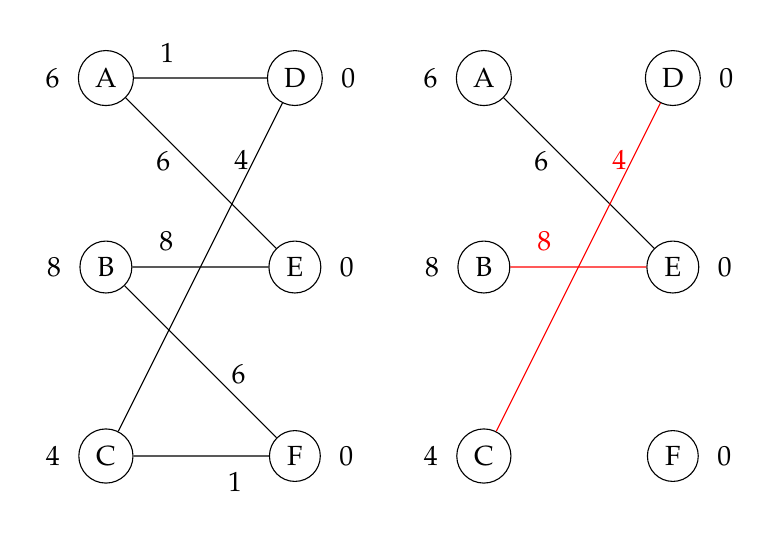
\begin{tikzpicture}[scale=.8,auto=left,every node/.style={circle,draw=black}]

			%left nodes
			\node [label=left:{6}] (n1) at (1,10) {A};
			\node [label=left:{8}] (n2) at (1,7) {B};
			\node [label=left:{4}] (n3) at (1,4) {C};

			%right nodes
			\node [label=right:{0}] (n4) at (4,10) {D};
			\node [label=right:{0}] (n5) at (4,7) {E};
			\node [label=right:{0}] (n6) at (4,4) {F};

			%edges
			\draw (n1) -- node[near start, draw=none, above] {1} ++ (n4);
			\draw (n1) -- node[near start, draw=none, below] {6} ++ (n5);
			\draw (n2) -- node[near start, draw=none, above] {8} ++ (n5);
			\draw (n2) -- node[near end, draw=none, above] {6} ++ (n6);
			\draw (n3) -- node[near end, draw=none, above] {4} ++ (n4);
			\draw (n3) -- node[near end, draw=none, below] {1} ++ (n6);

			
			
			%left nodes
			\node [label=left:{6}] (m1) at (7,10) {A};
			\node [label=left:{8}] (m2) at (7,7) {B};
			\node [label=left:{4}] (m3) at (7,4) {C};

			%right nodes
			\node [label=right:{0}] (m4) at (10,10) {D};
			\node [label=right:{0}] (m5) at (10,7) {E};
			\node [label=right:{0}] (m6) at (10,4) {F};
			
			%edges
			\draw (m1) -- node[near start, draw=none, below] {6} ++ (m5);
			\draw[red] (m2) -- node[near start, draw=none, above] {8} ++ (m5);
			\draw[red] (m3) -- node[near end, draw=none, above] {4} ++ (m4);
		\end{tikzpicture}
		\caption{Bipartite graph (left) and corresponding equality graph (right) with initial 
		matching}
	\end{figure}
	Our initial matching is $M = \{(B,E), (C,D)\}$ (see Figure 6). Note that the current state of 
	the graph is 
	primal-dual feasible. Our algorithm chooses an exposed vertex in $U$, say $A$. So we have 
	$S=\{A\}$ and $T=\emptyset$. We have that $N_l (S) \neq T$, so we find $E\in N_l (S)\setminus T
	$. $E$ is matched, so we grow our alternating tree as follows: $S := S\cup \{B\} = \{A,B\}$, 
	$T := T\cup \{E\} = \{E\}$. At this point $N_l (S) = T$, so we adjust our dual variables. 
	Calculate $\alpha = \min _{u\in S,v\notin T} \{l(u) + l(v) - w_{uv}\} = 2$ from edge $(B,F)$. 
	Our new equality graph is shown in Figure 7.
	\begin{figure}[H]
		\centering
		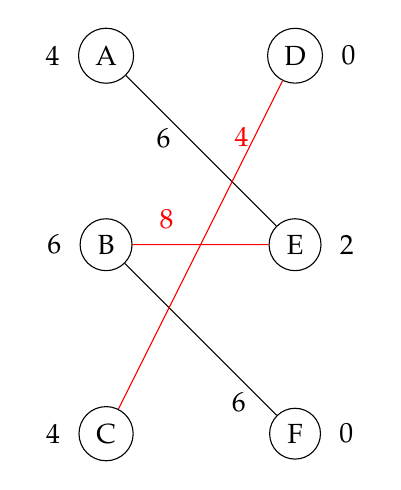
\begin{tikzpicture}[scale=.8,auto=left,every node/.style={circle,draw=black}]
			%left nodes
			\node [label=left:{4}] (m1) at (7,10) {A};
			\node [label=left:{6}] (m2) at (7,7) {B};
			\node [label=left:{4}] (m3) at (7,4) {C};

			%right nodes
			\node [label=right:{0}] (m4) at (10,10) {D};
			\node [label=right:{2}] (m5) at (10,7) {E};
			\node [label=right:{0}] (m6) at (10,4) {F};
			
			%edges
			\draw (m1) -- node[near start, draw=none, below] {6} ++ (m5);
			\draw[red] (m2) -- node[near start, draw=none, above] {8} ++ (m5);
			\draw (m2) -- node[near end, draw=none, below] {6} ++ (m6);
			\draw[red] (m3) -- node[near end, draw=none, above] {4} ++ (m4);
		\end{tikzpicture}
		\caption{Second equality graph.}
	\end{figure}
	Now, $S = \{A,B\}$ is the same, but $N_l (S) = \{E,F\}$ has changed. $T = \{E\}$, so 
	$N_l (S) \neq T$. So we choose $F\in N_l (S)\setminus T$. $F$ is unmatched, meaning it is 
	an endpoint of an augmenting path. In particular, $p = A,E,B,F$ is an augmenting path. Thus we 
	improve our matching with $M := M\oplus p = \{(A,E), (B,F), (C,D)\}$. Our equality graph with 
	the new matching is given in Figure 8.
	\begin{figure}[H]
		\centering
		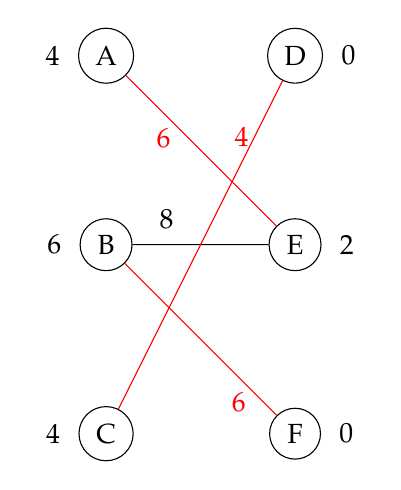
\begin{tikzpicture}[scale=.8,auto=left,every node/.style={circle,draw=black}]
			%left nodes
			\node [label=left:{4}] (m1) at (7,10) {A};
			\node [label=left:{6}] (m2) at (7,7) {B};
			\node [label=left:{4}] (m3) at (7,4) {C};

			%right nodes
			\node [label=right:{0}] (m4) at (10,10) {D};
			\node [label=right:{2}] (m5) at (10,7) {E};
			\node [label=right:{0}] (m6) at (10,4) {F};
			
			%edges
			\draw[red] (m1) -- node[near start, draw=none, below] {6} ++ (m5);
			\draw (m2) -- node[near start, draw=none, above] {8} ++ (m5);
			\draw[red] (m2) -- node[near end, draw=none, below] {6} ++ (m6);
			\draw[red] (m3) -- node[near end, draw=none, above] {4} ++ (m4);
		\end{tikzpicture}
		\caption{Equality graph after augmenting.}
	\end{figure}
	This is a perfect matching on the equality graph, so this matching must be a maximum weight 
	matching on the graph. We can check that the values of the primal and dual solutions agree. 
	The sum of weights in the matching is $6+6+4 = 16$, and the sum of the values of our 
	dual variables is $4+6+4+2 = 16$.\\
	Note that if we want to just find a maximum cardinality matching on a bipartite graph, 
	we can just give all edges weight 1 and run this algorithm.\\
	This algorithm was one of the first primal-dual algorithms developed, and it anticipated many 
	later variations on the same theme. It displays the surprising connection between combinatorial 
	optimization and linear programming, which we explore in the next section.
\end{section}
\end{document}
